\thispagestyle{toancuabinone}
\pagestyle{toancuabi}
\everymath{\color{toancuabi}}
%\blfootnote{$^1$\color{toancuabi}Đại học Thăng Long.}
\graphicspath{{../toancuabi/pic/}}
\begingroup
\AddToShipoutPicture*{\put(0,616){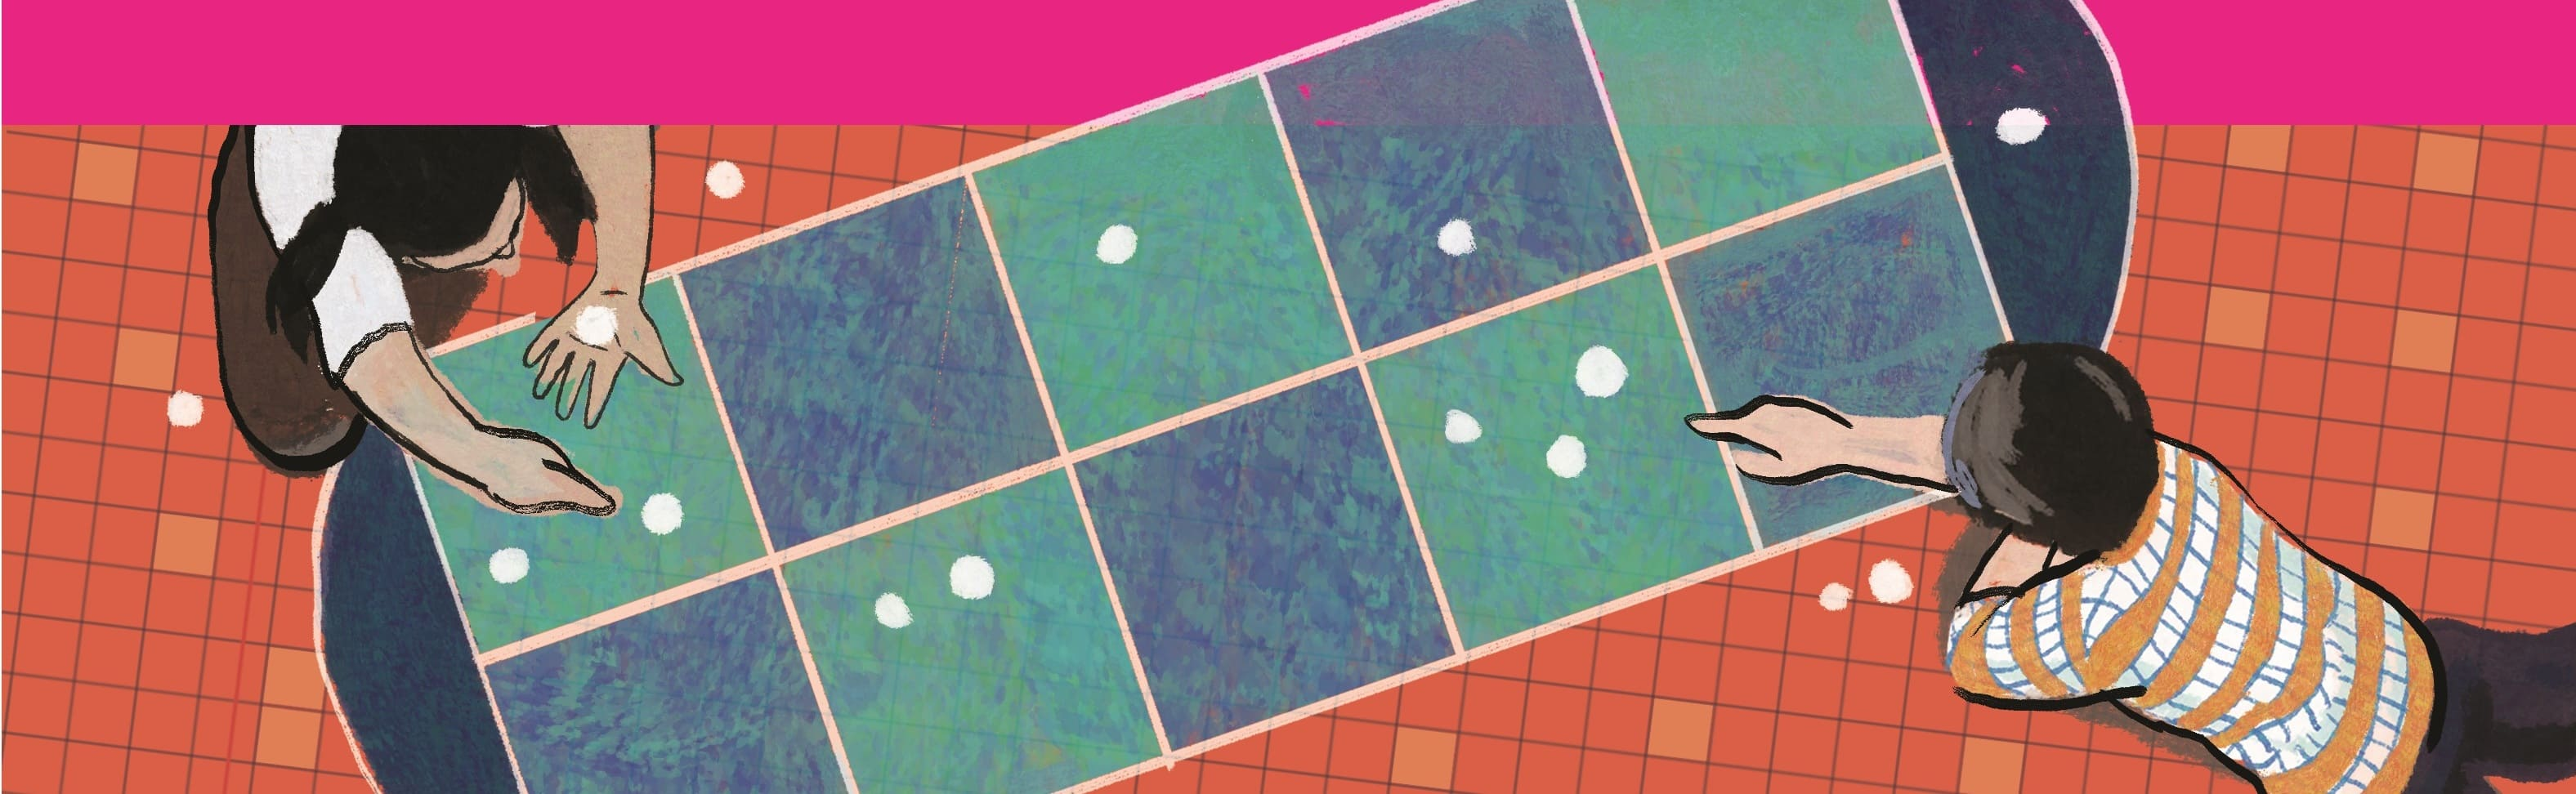
\includegraphics[width=19.3cm]{../bannertoancuabi}}}  
\AddToShipoutPicture*{\put(78,550){
\includegraphics[scale=1]{../tieude.pdf}}} 
\centering
\endgroup
\vspace*{160pt}

%\begin{multicols}{2}
%	Để điều tra một vụ án về kinh tế, Thám tử Xuân Phong cần thẩm vấn các đại diện của hai công ty vốn cạnh tranh kịch liệt với nhau là Sungsang và TungTeng. Qua thư ký bố trí xếp lịch, Xuân Phong mời được ba người là ông Kim, ông Lee và ông Han của hai công ty đình đám nọ tới văn phòng. Lịch sử cạnh tranh hàng chục năm nay của hai công ty này luôn chỉ ra rằng: các đại diện của cùng một công ty luôn nói thật với nhau, còn với đại diện của công ty cạnh tranh lại luôn \linebreak nói dối. 
%	\vskip 0.1cm
%	Các vị khách có mặt đúng giờ tại văn phòng thám tử  trong các bộ com--lê sang trọng xứng với đẳng cấp của đại diện cho các công ty hàng đầu về công nghệ. Vừa nhìn thấy  nhau, ông Kim đã  tiến tới trước mặt ông Lee và nói ``Tôi tới từ công ty Sungsang". Ông Lee trả lời ngay ``Ô thế à! Vậy là ông và ông Han cùng làm ở một công ty đấy!".
%	\vskip 0.1cm
%	Từ đoạn hội thoại trên, Xuân Phong xác định được ngay ông Han làm ở công ty nào. Em có thể lập luận xem làm cách nào mà thám tử lại biết vậy được không?
%%	Lời giải
%%	\vskip 0.1cm
%%	Các em xét hai trường hợp sau đây: ông Kim và ông Lee làm ở cùng một công ty hoặc họ làm ở hai công ty khác nhau.
%%	\vskip 0.1cm
%%	Trường hợp đầu tiên, nếu ông Kim và ông Lee cùng làm ở một công ty, thì do họ nói thật với nhau, suy ra ông Kim làm ở công ty Sungsang. Nhưng vì ông Lee cũng nói thật, suy ra ông Han và ông Kim cùng làm ở công ty Sungsang.
%%	\vskip 0.1cm
%%	Trường hợp thứ hai, nếu họ làm khác công ty, thì ông Kim đã nói dối ông Lee, vì thế thực ra ông Kim làm ở công ty TungTeng. Nhưng do ông Lee cũng nói dối ông Kim, nên ông Kim và ông Han phải làm ở các công ty khác nhau. Vì ông Kim làm việc ở công ty TungTeng, nên ông Han làm việc ở công ty Sungsang.
%%	\vskip 0.1cm
%%	Như vậy, trong mọi trường hợp, ông Han luôn làm việc ở công ty Sungsang.
%\end{multicols}
%	\begin{figure}[H]
%	\centering
%	\vspace*{-5pt}
%	\captionsetup{labelformat= empty, justification=centering}
%	\includegraphics[width=1\linewidth]{xuanphong}
%	\vspace*{-5pt}
%	\end{figure}
%\newpage
%\begingroup
%\AddToShipoutPicture*{\put(115,670){
\includegraphics[scale=1]{../tieude11.pdf}}} 
%\centering
%\endgroup
%\vspace*{33pt}
%
%\begin{multicols}{2}
%	$\pmb{1.}$	Bạn Công đã trả $24$ nghìn đồng để mua được $1$ cuốn vở, $2$ chiếc bút chì và $1$ cái tẩy. Bạn Nam thì trả tận $54$ nghìn đồng để mua được $2$ cuốn vở, $3$ chiếc bút chì và $3$ cái tẩy. Hỏi bạn An đã trả bao nhiêu tiền để mua được $2$ cuốn vở, $5$ chiếc bút chì và $1$ cái tẩy?
%	\begin{figure}[H]
%		\centering
%		\vspace*{-5pt}
%		\captionsetup{labelformat= empty, justification=centering}
%		\includegraphics[width=1\linewidth]{Pi3_bai1}
%		\vspace*{-10pt}
%	\end{figure}
%	$\pmb{2.}$ Bác Tuyết mang sữa đựng đầy trong hai chiếc thùng ra chợ bán. Lượng sữa trong thùng to nhiều gấp $3$ lần lượng sữa trong chiếc thùng nhỏ. Khi trong chiếc thùng nhỏ còn có $15$ lít sữa, còn thùng to còn $35$ lít sữa, bác Tuyết đổ dồn một lượng sữa từ thùng to cho đầy chiếc thùng nhỏ. Khi đó trong chiếc thùng to lượng sữa còn lại  đầy tới một nửa thùng. Hỏi bác Tuyết đã đổ bao nhiêu sữa từ thùng to sang thùng nhỏ, và dung tích của mỗi thùng là bao nhiêu?
%	\begin{figure}[H]
%		\centering
%		\vspace*{-10pt}
%		\captionsetup{labelformat= empty, justification=centering}
%		\includegraphics[width=0.75\linewidth]{Pi3_bai2}
%		\vspace*{-5pt}
%	\end{figure}
%	$\pmb{3.}$ Một tấn hoa quả được chở tới siêu thị: táo được đóng theo các thùng gỗ  $48$ kg/thùng, lê được đóng trong các thùng gỗ $20$ kg/thùng, mận đựng trong hộp giấy theo $14$ kg/hộp còn nho đựng trong các hộp giấy theo $10$ kg/hộp. Biết rằng số kg táo được chở tới nhiều gấp đôi số kg lê, còn số kg mận và nho là bằng nhau, hỏi số lượng mỗi loại hoa quả đã được vận chuyển tới cửa hàng là bao nhiêu?
%	\begin{figure}[H]
%		\centering
%		\vspace*{-5pt}
%		\captionsetup{labelformat= empty, justification=centering}
%		\includegraphics[width=1\linewidth]{Pi3_bai3}
%		\vspace*{-10pt}
%	\end{figure}
%	$\pmb{4.}$ Bạn An khởi hành đi bộ từ làng $A$ tới làng $B$ lúc $8$h sáng. Đồng thời vào lúc đó, bạn Bình cũng đi bộ từ làng $B$ tới làng $A$. Hai bạn đều đi với vận tốc không đổi, nhưng có thể không bằng nhau. Khi gặp nhau ở giữa đường, bạn An còn phải đi thêm $32$ phút nữa, còn Bình phải đi thêm $18$ phút nữa thì mới tới nơi. Hỏi hai bạn đã gặp nhau sau bao lâu tính từ lúc khởi hành?
%	\begin{figure}[H]
%		\centering
%		\vspace*{-5pt}
%		\captionsetup{labelformat= empty, justification=centering}
%		\includegraphics[width=1\linewidth]{Pi3_bai4}
%		\vspace*{-10pt}
%	\end{figure}
%	$\pmb{5.}$ Trong một cuộc thi thể thao do nhà vua Pháp tổ chức, $3$ chàng ngự lâm pháo thủ là Athos, Porthos và Aramis cùng D'Artagnan chia nhau bốn vị trí đầu tiên: $1$, $2$, $3$, $4$ (ứng với giải thưởng: nhất, nhì, ba, bốn). Tổng ba số chỉ vị trí mà Athos, Porthos và D'Artagnan giữ là bằng $6$. Tổng hai số chỉ vị trí mà Porthos và Aramis giữ cũng bằng $6$. Hỏi mỗi chàng ngự lâm đã chiếm các giải nào, biết Porthos chiếm được giải cao hơn Arthos?
%	\begin{figure}[H]
%		\centering
%		\vspace*{-5pt}
%		\captionsetup{labelformat= empty, justification=centering}
%		\includegraphics[width=1\linewidth]{Pi3_bai5}
%		\vspace*{-15pt}
%	\end{figure}
%	$\pmb{6.}$ Tại một khách sạn nọ, nhân viên trực quản lý điều hành phải làm việc từ $8$h sáng tới $8$h tối (phương án $A$), hoặc từ $8$h tối tới $8$h sáng (phương án $B$), hoặc làm trọn cả ngày $24$h bắt đầu từ $8$h (sáng hoặc tối) (phương án $C$). Nếu làm theo phương án $A$, nhân viên trực quản lý sẽ được nghỉ không ít hơn $1$ ngày ($24$h). Nếu làm theo phương án $B$, nhân viên trực quản lý sẽ được nghỉ không ít hơn $1$ ngày rưỡi ($36$h). Còn nếu làm theo phương án $C$, nhân viên trực quản lý sẽ được nghỉ không ít hơn hai ngày rưỡi ($60$h).
%	\vskip 0.1cm
%	Hỏi khách sạn phải cần có ít nhất bao nhiêu nhân viên trực quản lý để đảm bảo lịch làm việc, nghỉ ngơi ở trên được tuân thủ?
%\end{multicols}
%\vspace*{-10pt}
%{\color{toancuabi}\rule{1\linewidth}{0.1pt}}
%\begingroup
%\AddToShipoutPicture*{\put(110,405){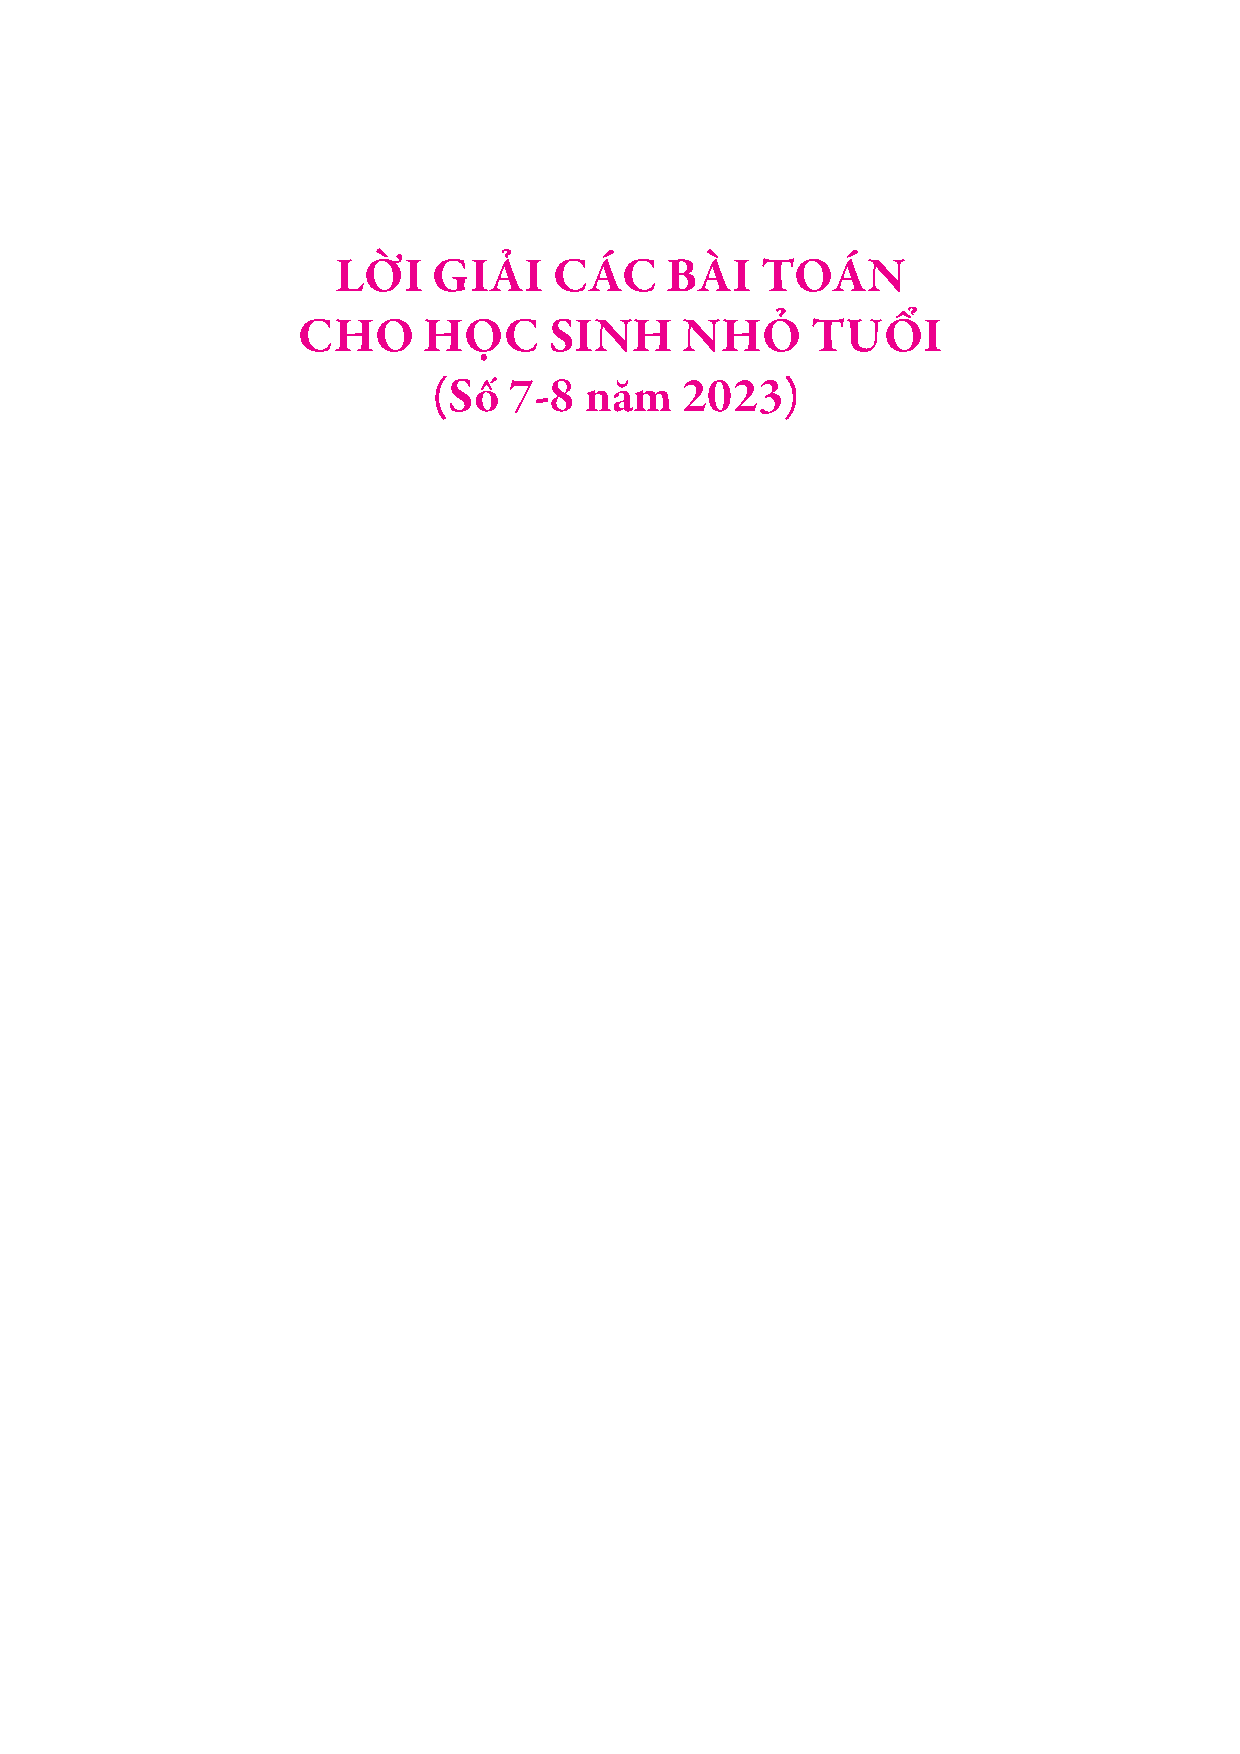
\includegraphics[scale=1]{../tieude2.pdf}}} 
%\centering
%\endgroup
%\vspace*{75pt}
%
%\begin{multicols}{2}
%	$\pmb{1.}$ Hai anh bạn rủ nhau đi câu cá. Khi được hỏi ``Trong mỗi giỏ của các anh có bao nhiêu con cá đấy?" thì anh thứ nhất trả lời ``Trong giỏ của tôi có số cá bằng nửa số cá ở giỏ của anh kia và thêm $10$ con nữa". Anh thứ hai lại nói ``Còn trong giỏ của tôi có số cá bằng số cá trong giỏ của anh kia và thêm $20$ con nữa". Vậy cả hai anh bạn có tất cả bao nhiêu con cá nhỉ? 
%	\begin{figure}[H]
%		\centering
%		\vspace*{-10pt}
%		\captionsetup{labelformat= empty, justification=centering}
%		\includegraphics[width=1\linewidth]{Pi10_ToanBi_Bai1}
%		\vspace*{-15pt}
%	\end{figure}
%	\textit{Lời giải.} Một nửa số cá của anh thứ hai sẽ là nửa số cá của anh thứ nhất cộng thêm $10$ con. Vậy nửa số cá của anh thứ hai cộng thêm $10$ con sẽ bằng nửa số cá của anh thứ nhất cộng thêm $20$ con. Theo đề bài, số cá này bằng cả số cá của anh thứ nhất.
%	\vskip 0.1cm
%	Vậy một nửa số cá của anh thứ nhất là: $20$ (con)
%	\vskip 0.1cm
%	Suy ra anh thứ nhất có số cá là
%	\begin{align*}
%		2 \times 20 = 40 \text{  (con)}
%	\end{align*}
%	và anh thứ hai có số cá là 
%	\begin{align*}
%		40+20 = 60 \text{  (con).}
%	\end{align*} 
%	Tổng số cá của cả hai anh là 
%	\begin{align*}
%		40+60 = 100 \text{  (con).}
%	\end{align*}
%	Đây là bài tập đơn giản, tuy nhiên các em thử tập làm bằng nhiều cách khác nhau thông qua suy luận thông thường mà không cần dùng tới cách lập phương trình nhé.
%	\vskip 0.1cm
%	$\pmb{2.}$ Lọ lem có $100$ rổ đựng hạt dẻ, lúc đầu số hạt dẻ trong mỗi rổ là như nhau. Lọ Lem lấy đi trong rổ thứ nhất một số hạt dẻ, lấy từ rổ  thứ hai một số hạt gấp đôi như thế, lấy từ rổ thứ ba một số hạt gấp ba như thế, và cứ như vậy. Cuối cùng thì trong rổ thứ $100$ chỉ còn đúng một hạt dẻ, và còn lại ở tất cả trong $100$ rổ tổng cộng là $14950$ hạt dẻ. Hỏi ban đầu trong mỗi rổ có bao nhiêu hạt dẻ?
%	\begin{figure}[H]
%		\centering
%		\vspace*{-10pt}
%		\captionsetup{labelformat= empty, justification=centering}
%		\includegraphics[width=1\linewidth]{Pi10_ToanBi_Bai2}
%		\vspace*{-15pt}
%	\end{figure}
%	\textit{Lời giải.} 	Gọi số hạt dẻ mà Lọ Lem lấy ở rổ thứ nhất là $a$, khi đó tổng cộng số hạt dẻ mà Lọ lem đã lấy đi ở $100$ rổ là
%	\begin{align*}
%		a+ 2a+\cdots+100a=5050a.
%	\end{align*} 
%	Do rổ cuối cùng còn lại $1$ hạt dẻ nên ban đầu số hạt dẻ ở rổ cuối cùng (cũng là số hạt dẻ ở các rổ khác) là: $100a+1$ (hạt).
%	\vskip 0.1cm
%	Vậy, ban đầu tổng số hạt dẻ là
%	\begin{align*}
%		100\times(100a+1) = 10000a+100 \text{  (hạt).}
%	\end{align*} 
%	Ta có hệ thức là: $10000a+100-5050 a =14950$. Từ đó suy ra $a=3$. Vì vậy ban đầu mỗi rổ có  $100\times 3+1 = 301$ hạt dẻ.
%	\vskip 0.1cm
%	$\pmb{3.}$ Hai bạn học sinh là Nam và Vũ gặp nhau tại nhà của Vũ. Nam nói ``Nếu lấy số nhà của tớ là một số có hai chữ số trừ đi số có hai chữ số tạo thành khi viết theo thứ tự ngược lại, thì sẽ ra số nhà của cậu. Vậy tớ sống ở số nhà nào?"
%	\vskip 0.1cm
%	Vũ trả lời ``Ôi, bài toán này dễ quá" -- và giải ra luôn đáp số.
%	\vskip 0.1cm
%	Vậy các bạn đó sống ở những số nhà nào nhỉ?
%	\vskip 0.1cm
%	\textit{Lời giải.} 	Nếu thực hiện phép trừ của Nam, ta sẽ nhận được số có dạng $9\times k$, ở đó $k$ là hiệu của chữ số hàng chục và chữ số hàng đơn vị. Vì số viết theo thứ tự ngược lại cũng là số có hai chữ số, nên $k\le8$. 
%	\vskip 0.1cm
%	Nếu $k<8$ thì có thể thấy có nhiều số có hai chữ số (là số nhà) mà sau khi làm phép tính trừ đã cho sẽ cho kết quả như nhau. Khi đó Vũ không thể giải được ngay câu đố của Nam. Do đó $k=8$. Các em có thể tìm thấy số nhà của Nam là $91$, và số nhà của Vũ là $72$.
%	\begin{figure}[H]
%		\centering
%		\vspace*{-5pt}
%		\captionsetup{labelformat= empty, justification=centering}
%		\includegraphics[width=1\linewidth]{Pi10_ToanBi_Bai3}
%		\vspace*{-15pt}
%	\end{figure}
%	$\pmb{4.}$ Lớp của Hùng có $35$ học sinh. Trong số đó có $20$ em tham gia câu lạc bộ Toán, $11$ em tham gia câu lạc bộ Khéo tay, $10$ em không tham gia vào hai nhóm này. Hỏi có tất cả bao nhiêu em vừa tham gia CLB Toán lại vẫn không quên tham gia cả CLB Khéo tay nhỉ?
%	\begin{figure}[H]
%		\centering
%		\vspace*{-5pt}
%		\captionsetup{labelformat= empty, justification=centering}
%		\includegraphics[width=1\linewidth]{Pi10_ToanBi_Bai4}
%		\vspace*{-15pt}
%	\end{figure}
%	\textit{Lời giải.} 	Chúng ta chia toàn bộ số học sinh trong lớp thành bốn danh sách, mà không có em nào ở trong hai danh sách khác nhau, như sau. Danh sách ``toán thuần tuý" gồm các bạn chỉ tham gia CLB Toán, danh sách ``khéo tay thuần tuý" gồm các bạn chỉ tham gia CLB Khéo tay, danh sách ``giỏi toán lại khéo tay" gồm các bạn tham gia cả $2$ CLB  và cuối cùng là danh sách ``rảnh rỗi" là các bạn không tham gia vào hai CLB này. Theo đề bài, danh sách ``rảnh rỗi" có $10$ bạn, vì thế có $25$ bạn không ``rảnh rỗi". Trong số $25$ bạn này có $20$ bạn tham gia nhóm Toán, vì thế số ``khéo tay thuần tuý" là $5$ bạn. Vậy số bạn vừa tham gia nhóm Toán lại ``khéo tay" nữa là 
%	\begin{align*}
%		11-5 = 6 \text{ (bạn).}
%	\end{align*}
%	$\pmb{5.}$ Tùng đến trường mới có nhiều chuyện rất vui nên về khoe với bạn bè.
%	\begin{figure}[H]
%		\centering
%		%		\vspace*{5pt}
%		\captionsetup{labelformat= empty, justification=centering}
%		\includegraphics[width=1\linewidth]{Pi10_ToanBi_Bai5}
%		\vspace*{-15pt}
%	\end{figure}
%	-- Lớp tớ có $35$ học sinh. Và các cậu có tưởng tượng được không, mỗi người lại kết bạn với đúng $11$ học sinh cùng lớp.
%	\vskip 0.1cm
%	-- Không thể thế được! Bách, người bạn thân của Tùng vừa đạt giải trong một cuộc thi Olympic, ngay lập tức trả lời.
%	\vskip 0.1cm
%	Vì sao Bách lại nghĩ như vậy nhỉ?
%	\vskip 0.1cm
%	\textit{Lời giải.} 	Ta biểu diễn mỗi học sinh được thể hiện bởi một điểm. Nếu hai học sinh kết bạn với nhau ta sẽ nối hai điểm tương ứng bởi một đoạn thẳng. Như vậy có $35$ điểm, mỗi điểm được nối đúng với $11$ điểm khác. Khi đó tổng số các đầu của các đoạn thẳng nối quan hệ bạn bè là $35\times11$ là một số lẻ. Điều này là vô lý do mỗi đoạn thẳng thể hiện quan hệ bạn bè có đúng hai điểm đầu mút. 
%	\vskip 0.1cm
%	$\pmb{6.}$ Có $55$ em học sinh tham gia một cuộc thi Olympic. Tất cả các em đều nộp bài. Khi chấm bài, mỗi câu hỏi được chấm bởi một trong ba loại điểm: điểm ``$+$" nếu câu hỏi được trả lời hoàn toàn đúng; điểm ``$-$" nếu câu hỏi đã có trả lời nhưng chưa ra đúng đáp số; và điểm ``$0$" nếu câu hỏi chưa được trả lời. Sau khi chấm toàn bộ bài thi, ban tổ chức thấy không có hai bài thi nào có cả các số điểm ``$+$" và số điểm ``$-$" đồng thời trùng nhau. Vậy trong kỳ thi Olympic đó phải có ít nhất bao nhiêu câu hỏi?
%	\vskip 0.1cm
%	\textit{Lời giải.} 	Giả sử $a$ là số câu hỏi được ra.  Ta chia ra các trường hợp sau
%	\vskip 0.1cm
%	$1.$ Bài thi có tất cả các câu hỏi đều được trả lời: Khi đó số các bài thi sẽ không vượt quá $a+1$ bài: từ bài có $a$ dâú ``$+$" và $0$ dấu ``$-$" cho đến bài có $0$ dấu ``$+$" và $a$ dấu ``$-$".  
%	\vskip 0.1cm
%	Bài thi trong đó chỉ có đúng một bài chưa có trả lời (có một điểm ``$0$"): Số các bài thi  nhiều nhất là $a$ bài (từ $a-1$ điểm ``$+$" và $0$ điểm ``$-$" cho đến bài có $0$ điểm ``$+$" và $a-1$ điểm ``$-$"). $\ldots$
%	\vskip 0.1cm
%	Và cứ xét như vậy, ta thấy tổng số các bài thi nhiều nhất là 
%	\begin{align*}
%		(a\!+\!1)\!+\!a\!+\!(a\!-\!1)\!+\!\cdots\!+\!1=\dfrac{(a\!+\!1)(a\!+\!2)}{2}.
%	\end{align*}
%	Từ đó ta có $55\le\dfrac{(a+1)(a+2)}{2}$. Với $a=9$ ta có $\dfrac{10\cdot11}{2}=55$. Vậy là $a \ge 9$. 
%	\vskip 0.1cm
%	Vì vậy số câu hỏi ít nhất được ra là $9$ câu.
%\end{multicols}
\newpage
\begingroup
\thispagestyle{toancuabinone}
\blfootnote{$^1$\color{toancuabi}Ottawa, Canada.}
\AddToShipoutPicture*{\put(60,733){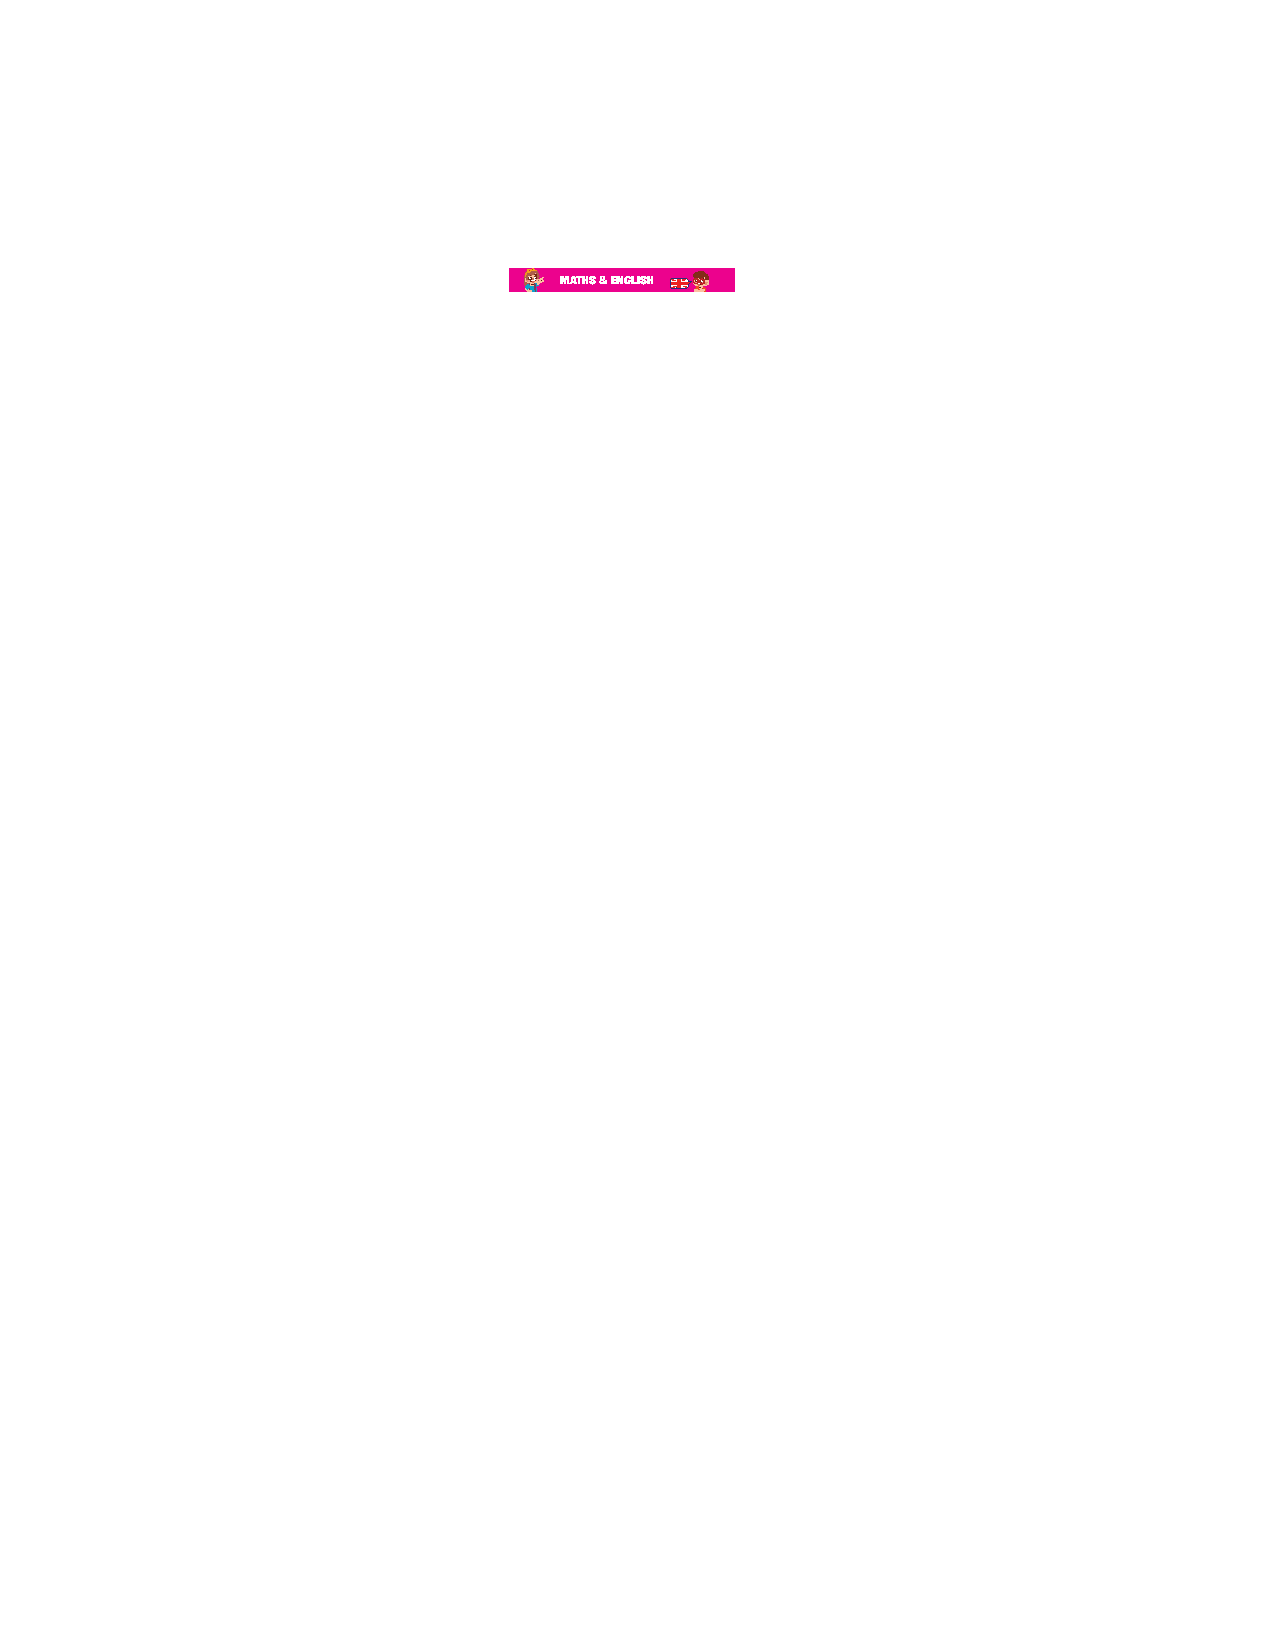
\includegraphics[width=17.2cm]{../mathc.pdf}}}
%\AddToShipoutPicture*{\put(-2,733){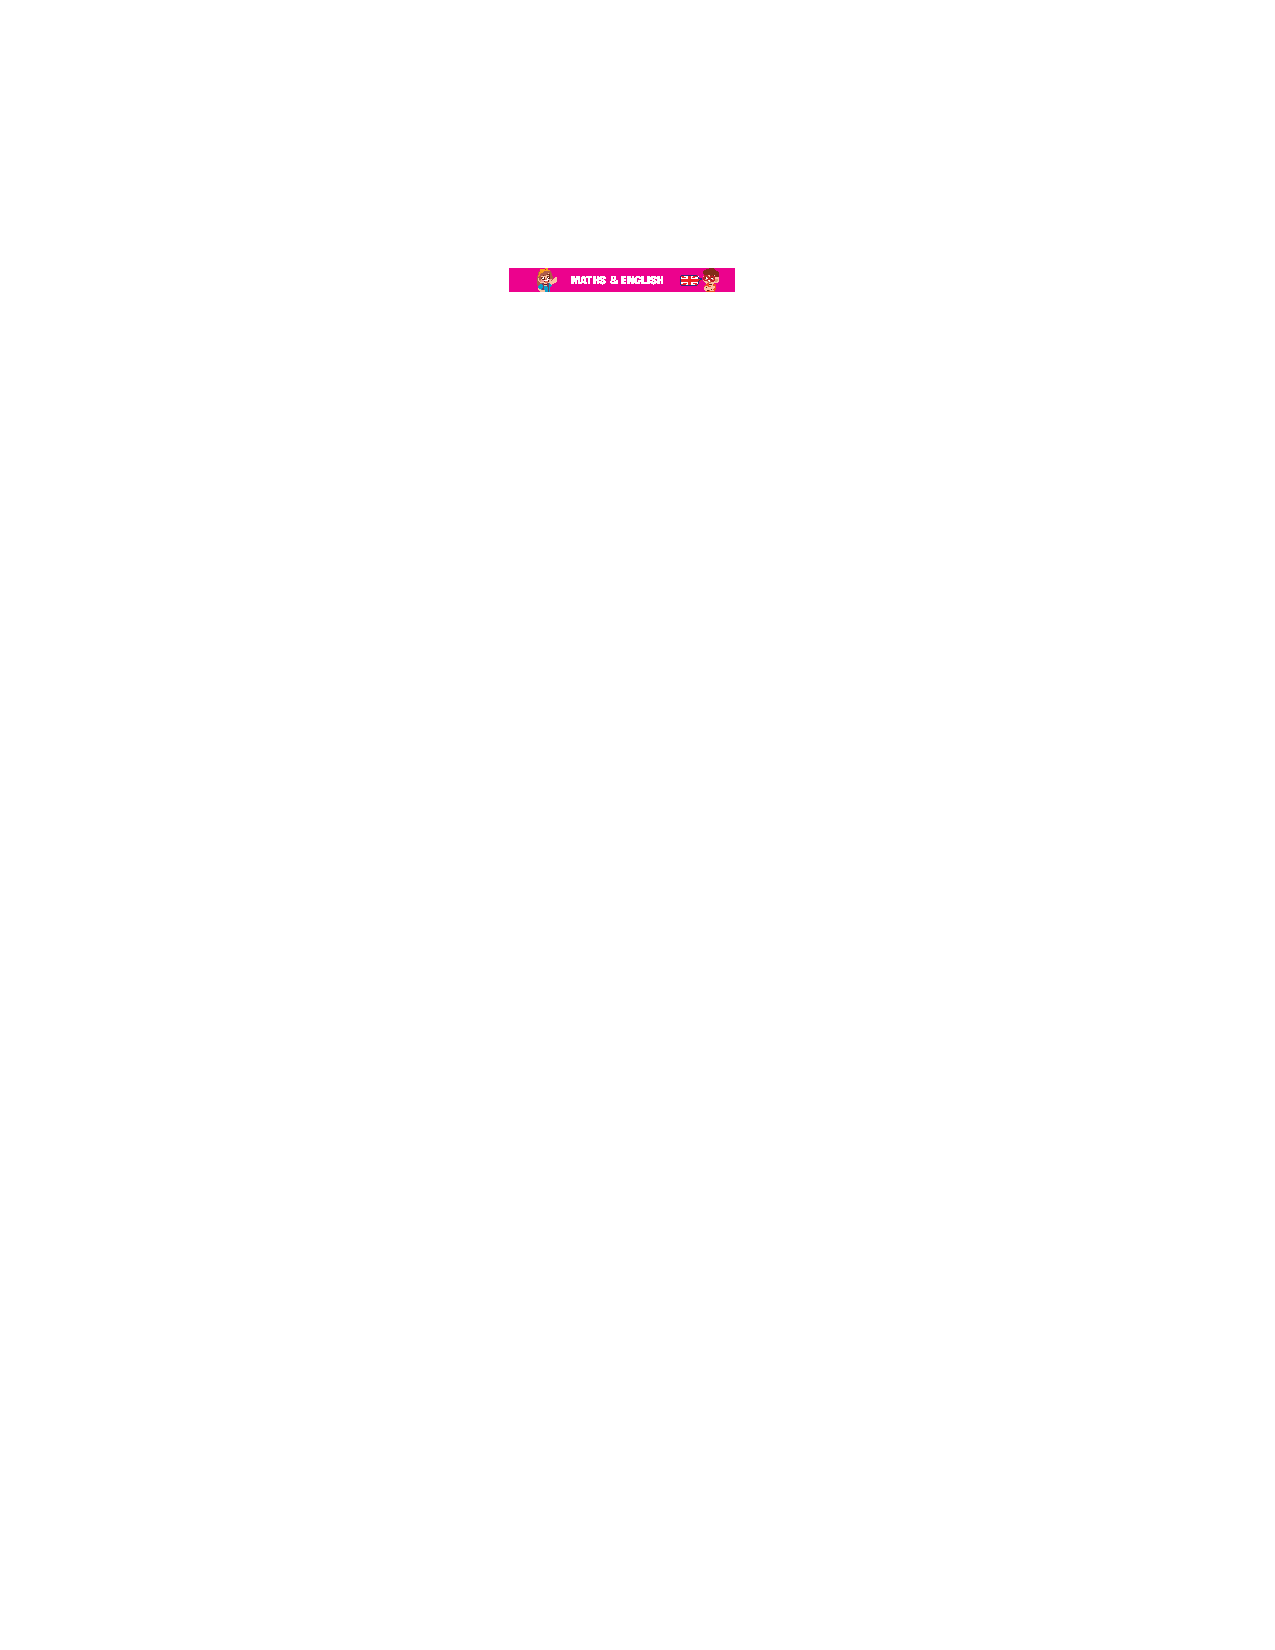
\includegraphics[width=17.2cm]{../mathl.pdf}}} 
\AddToShipoutPicture*{\put(170,675){
\includegraphics[scale=1]{../tieude4.pdf}}} 
\centering
\endgroup
\graphicspath{{../toancuabi/pic/}}
\vspace*{33pt}

\begin{multicols}{2}
	In this article, we explore the use of Venn diagrams through a few examples.
	\vskip 0.2cm
	\PIbox{{\color{toancuabi}\textbf{Example} (Overlapping rugs)\textbf{.}}
		Three rugs have a combined area of $200$ $m^2.$ The rugs are overlapped as shown in the diagram below.
		The overlapped rugs together cover a floor area of $140$ $m^2.$ Furthermore the area covered by exactly any two rugs is $24$ $m^2$. 
		What is the are of floor is covered by all three rugs?}
	\begin{figure}[H]
		\vspace*{-5pt}
		\centering
		\captionsetup{labelformat= empty, justification=centering}
		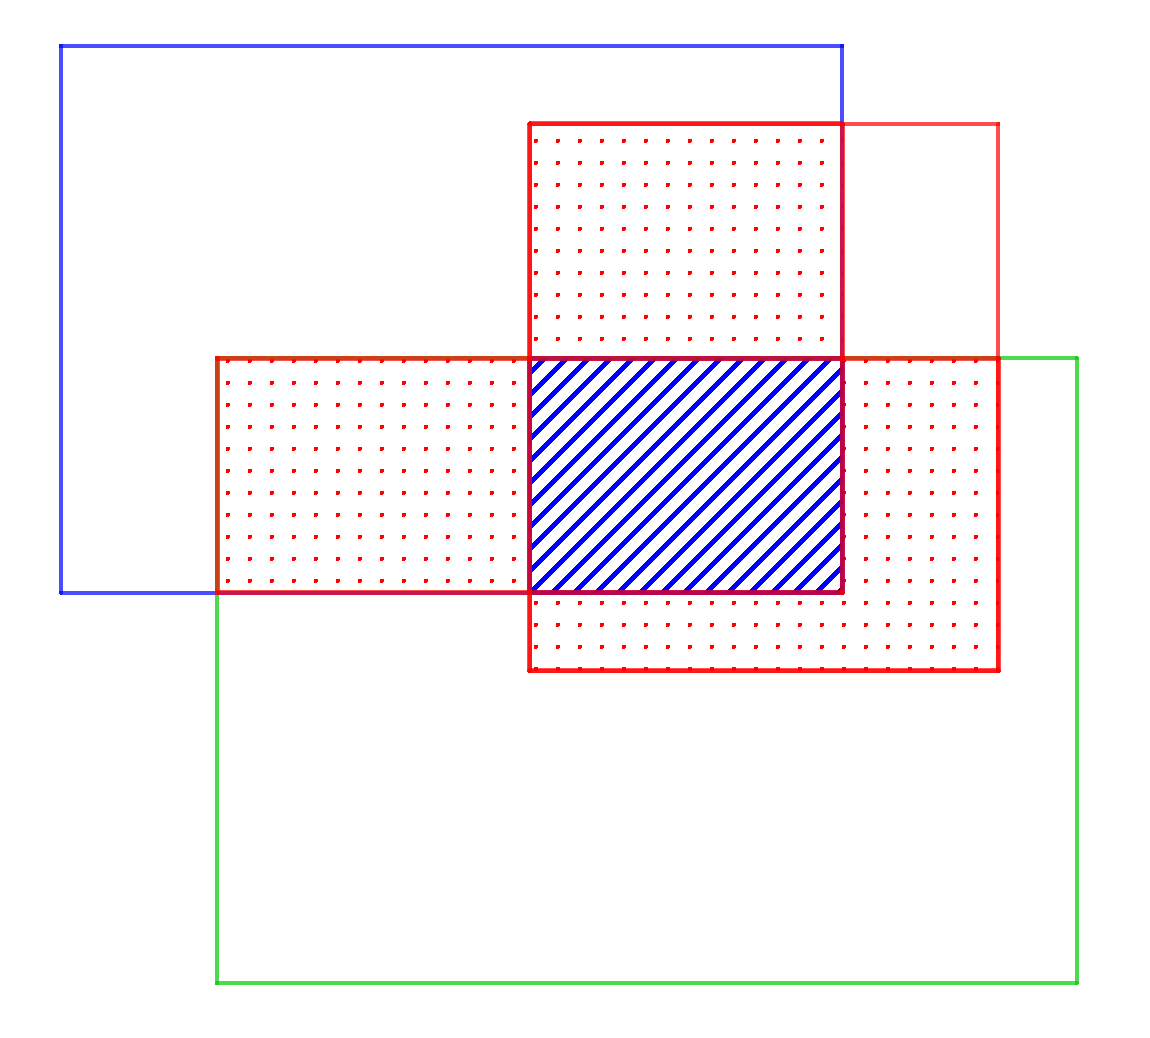
\includegraphics[width= 1\linewidth]{pi-2023-01-01.pdf}
		\vspace*{-15pt}
	\end{figure}
	\textit{Solution.}
	The total area of the three rugs, when not overlapping, is the sum of the areas of the three rectangles, which is $200$ $m^2.$
	The region show in the diagram above, formed by the overlapping rugs, has a total area of $140$ $m^2.$
	This means that $200-140=60$ $m^2$ is the total area of the three \textcolor{red}{red dotted parts},
	(because they are where the rugs overlapped once) plus twice \textcolor{blue}{the blue hatch part},
	(because it is where the rugs overlapped twice).
	\vskip 0.1cm
	In other words, if $r$ and $b$ are the areas of a red dotted and the blue hatch, respectively, then $3r + 2b = 60.$
	Furthermore, note that the area of a red dotted part plus the blue hatch part is $24$ $m^2,$ thus $r + b = 24.$
	Therefore $b = 3(r + b)- (3r+2b) = 3 \cdot 24 - 60 = 12.$
	\vskip 0.2cm
	\PIbox{
	{\color{toancuabi}\textbf{Exercise} (Overlapping circles)\textbf{.}}
		Three circles with radius $2, 3$ and $4$ are overlapping each other.
		The largest circle is partitioned into shaded region A and unshaded regions B and C.
		If the total area of the shaded region is $17\pi,$ what is the area of region A in terms of $\pi$?}
	\begin{figure}[H]
		\vspace*{-5pt}
		\centering
		\captionsetup{labelformat= empty, justification=centering}
		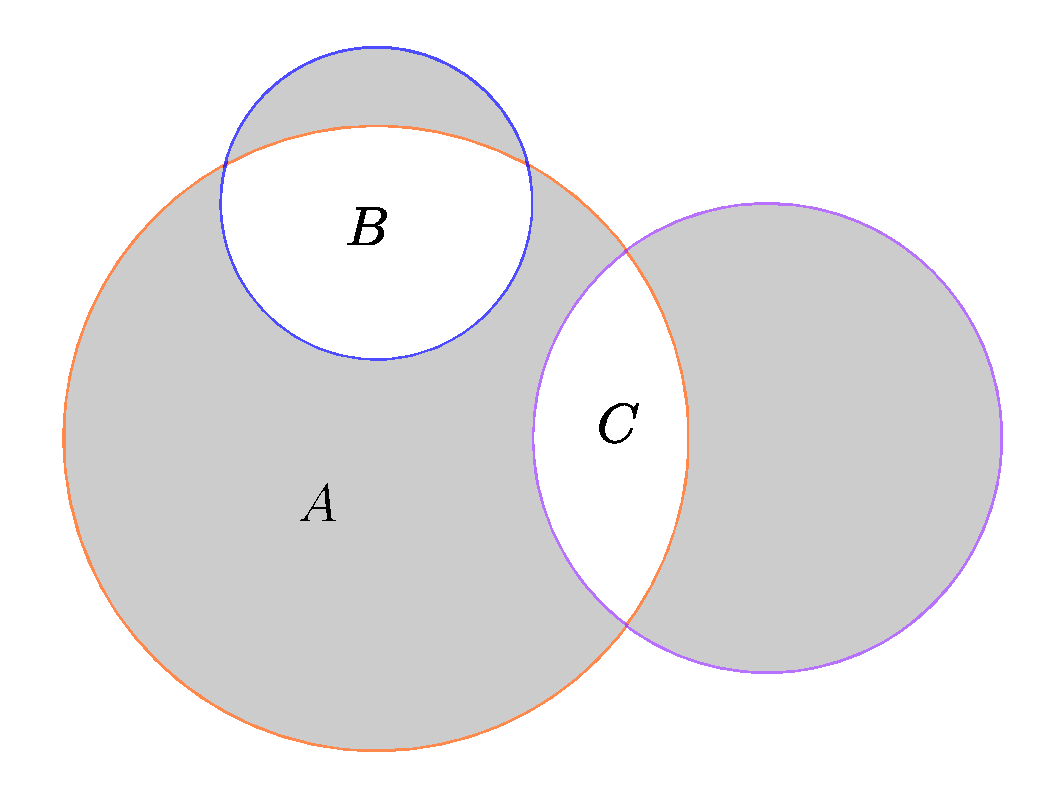
\includegraphics[width= 1\linewidth]{pi-2023-01-02.pdf}
		\vspace*{-15pt}
	\end{figure}
	\textit{Solution.}
	The total area of the circles is the area of the shaded region plus \textit{twice} the area of the unshaded regions:
	\begin{align*}
		&4\pi + 9\pi + 16\pi = 17\pi + 2(B+C) \\
		\Rightarrow \,&B+C = 6\pi \\
		\Rightarrow \,&A = 16\pi - (B+C) = 10\pi
	\end{align*}
	\vskip 0.1cm
	\PIbox{{\color{toancuabi}\textbf{Example} (Alligators are ferocious and creepy crawlers)\textbf{.}}
	If all alligators are ferocious creatures and some creepy crawlers are alligators. It is easy to verify that:
	(i) all alligators are creepy crawlers; (ii) some ferocious creatures are creepy crawlers;
	and (iii) some alligators are not creepy creatures.}
	
	\PIbox{
	Now, which statements below are true, false, or undecidable (you can't say it is true or false)?
	\vskip 0.1cm
	$S1.$ Some of creepy creatures are ferocious.
	\vskip 0.1cm
	$S2.$ Some ferocious creatures are creepy crawlers.
	\vskip 0.1cm
	$S3.$ Some alligators are not creepy creatures.
	\vskip 0.1cm
	$S4.$ Some ferocious crawlers are not alligators.
	\vskip 0.1cm
	$S5.$ Alligators are ferocious and creepy crawlers.}
	\vskip 0.1cm
	\textit{Solution.}
	To help the reasoning with visual cues, you can use Venn diagrams.
	\vskip 0.1cm
	First, we draw a \textcolor{red}{circle} depicting the set of alligators. In other words all alligators are in this circle.
	Since all alligators are ferocious creatures, thus the \textcolor{blue}{circle} containing all ferocious creatures must cover the circle of alligators .
	Now, some creepy crawlers are alligators, thus the \textcolor{green}{circle} containing all creepy crawlers must intersect and not contain the circle of alligators.
	Logically the circle of creepy crawlers then should intersect the circle of ferocious creatures and should not cover it.
	We got the diagram shown below.
	\begin{figure}[H]
		\vspace*{-5pt}
		\centering
		\captionsetup{labelformat= empty, justification=centering}
		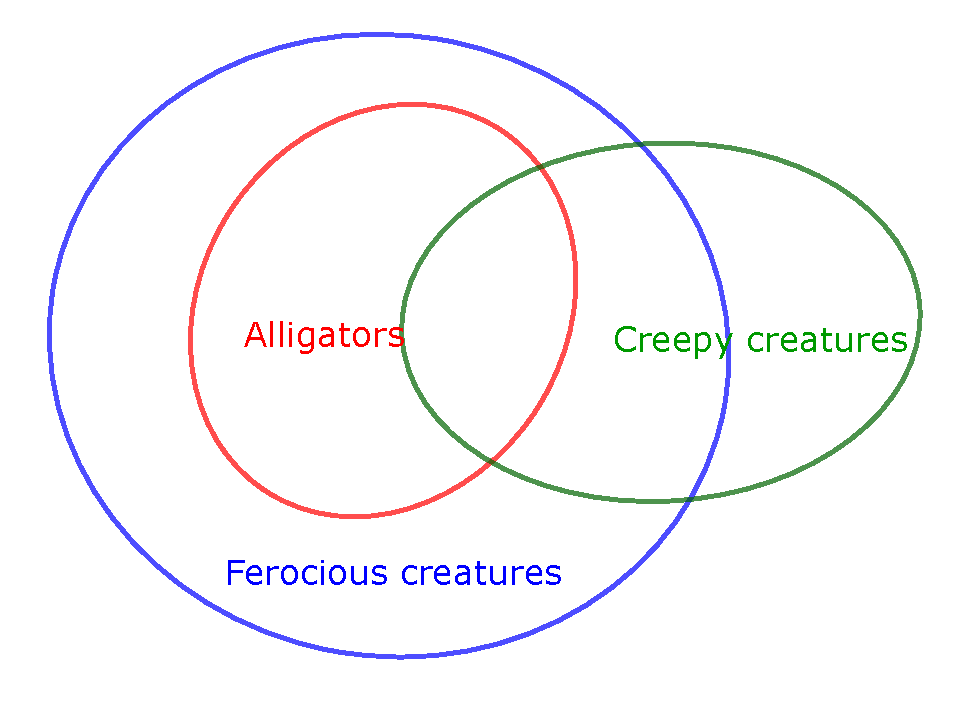
\includegraphics[width= 1\linewidth]{pi-2023-01-03.pdf}
		\vspace*{-10pt}
	\end{figure}
	For $S1,$ those creepy crawlers are alligators, they must be in the intersection of the \textcolor{red}{circle} and \textcolor{green}{circle}.
	Since the \textcolor{red}{circle} resides within of the \textcolor{blue}{circle} the intersection must be part of the \textcolor{blue}{circle}.
	In other words those creepy crawlers are ferocious creatures. Thus the statement $B1$ is true.
	\vskip 0.1cm
	It is also easy to verify that $S2$ is true.
	\vskip 0.1cm
	Since we know that \textit{some creepy crawlers are alligators}, thus the \textcolor{green}{circle} intersect
	and may not contain the whole the \textcolor{red}{circle}, thus $S2$ is \textit{undecidable.}
	We don't know if some alligators are cute and not creepy.
	\vskip 0.1cm
	The remaining two statements $S4$ and $S5$ are both \textit{undecidable}. Try to prove it yourself.
	\vskip 0.1cm
	\PIbox{{\color{toancuabi}\textbf{Exercise} (Are boys good at math)\textbf{.}}
		Let assume that \textit{all boys in the math club are good at math.} 
		Which of the following statements must be true?
		\vskip 0.1cm
		$S1.$ No boy whose math is not good is a member of the math club.
		\vskip 0.1cm
		$S2.$ All boys whose math is good are members of the math club.
		\vskip 0.1cm
		$S3.$ All boys who are not members of the math club are not good at math.
		\vskip 0.1cm
		$S4.$ Every member of the math club whose math is good is a boy.
		\vskip 0.1cm
		$S5.$ There is one boy in the math club whose math is not good.
		\vskip 0.1cm
		Now decide that the following is true or false.
		\textit{A girl is good at math as a boy who is not member of the math club is not good as math as a boy who is member of the math club.}}
	\vskip 0.1cm
	\textit{Solution.}
		Draw three circles pairwise--intersecting each other, one labeled \textit{boys} (the girls are outside of this circle),
		the second other one labeled \textit{math} meaning whoever in this circle is good at math (the ones out side of it are not),
		and the third one labeled \textit{club} meaning whoever in this circle is member of the math club (the ones out side of it are not).
		None of the circle can contain another one. The club circle must cover the intersection of the boys and the math circle.
		A diagram is shown as below.
		\begin{figure}[H]
%			\vspace*{-5pt}
			\centering
			\captionsetup{labelformat= empty, justification=centering}
			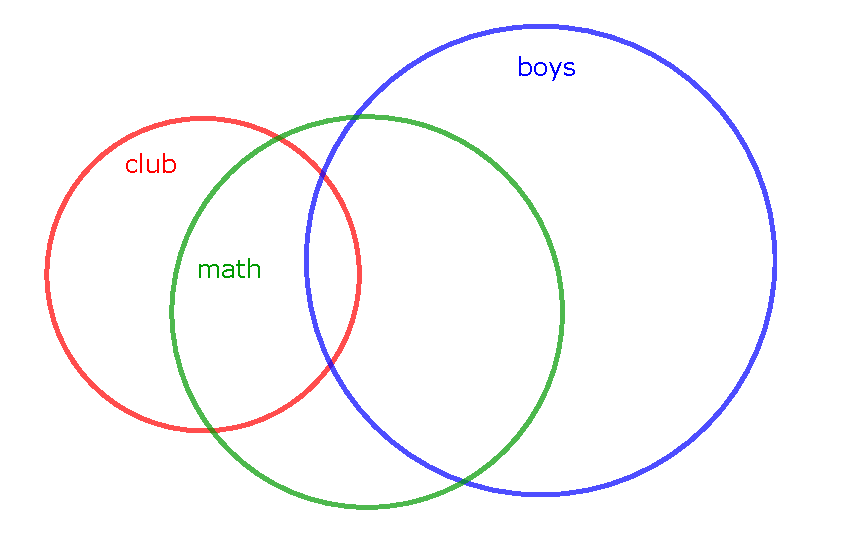
\includegraphics[width= 1\linewidth]{pi-2023-01-04.pdf}
			\vspace*{-10pt}
		\end{figure}
		For $S2,S3, S4,$ and $S5,$ it is easy to find a counter example, thus none of them is true.
		$S1$ is true, otherwise if there were a boy whose math is not good and is a member of the math club,
		then because he is a member of the math club, his math has to be good. This contracdiction means the statement is true.
\end{multicols}
	